\section{Processus max-stables}

Cette partie constitue le cœur du passage de la théorie des valeurs extrêmes
univariée à sa version spatiale. L'idée directrice tient en une phrase :
\emph{un processus max-stable est à un champ spatial ce que la loi GEV est à une
seule variable}. Là où le cours donne la loi du maximum en un point, on décrit
ici le comportement conjoint des maxima en tout point d'une région.

\subsection{Définition et convergence}

On note $\bigvee$ le supremum et $\overset{d}{=}$, $\overset{d}{\to}$ l'égalité
et la convergence en loi.

\begin{definition}[Processus max-stable]
Un processus stochastique $\{G(\mathbf x)\}_{\mathbf x\in\R^d}$ est
\emph{max-stable} s'il existe des suites de fonctions continues
$a_T(\mathbf x)>0$ et $b_T(\mathbf x)$ telles que, pour des répliques
indépendantes $G_1,\dots,G_T$ de $G$,
\[
\left\{\frac{\bigvee_{t=1}^T G_t(\mathbf x)-b_T(\mathbf x)}{a_T(\mathbf x)}\right\}_{\mathbf x\in\R^d}
\;\overset{d}{=}\; \{G(\mathbf x)\}_{\mathbf x\in\R^d}.
\]
\end{definition}

Autrement dit, prendre le maximum ponctuel de plusieurs copies indépendantes,
puis renormaliser, redonne le même processus en loi. C'est la propriété de
max-stabilité du cours, mais portée par un \emph{champ} tout entier et non plus
par un nombre.

Le résultat fondamental justifie l'emploi de ces processus : si le maximum
ponctuel renormalisé de $n$ répliques indépendantes d'un processus quelconque
converge vers un processus non dégénéré, alors ce processus limite est
\emph{nécessairement} max-stable :
\begin{equation}\label{eq:conv-ms}
\left\{\frac{\bigvee_{i=1}^n \{T_i(\mathbf x)\}-d_n(\mathbf x)}{c_n(\mathbf x)}\right\}_{\mathbf x}
\;\overset{d}{\to}\; \{G(\mathbf x)\}_{\mathbf x},\qquad n\to\infty
\end{equation}
(de Haan, 1984). C'est l'analogue spatial exact du théorème de
Fisher--Tippett--Gnedenko : de même que la GEV est la seule limite possible du
maximum d'une variable, le processus max-stable est la seule limite possible du
maximum d'un champ. En pratique, le nombre $n$ d'observations sur lequel on
prend le maximum dépend de la période considérée (classiquement $T_L=1$ an,
$n=365$).

On appelle \emph{simple} un processus max-stable dont les marges sont de
Fréchet standard, c'est-à-dire $\PP(Z(\mathbf x)\le z)=\exp(-1/z)$ en chaque
point $\mathbf x$. C'est le cadre de tout ce qui suit.

\subsection{Représentation spectrale}

Comment fabriquer concrètement de tels processus ? La \emph{représentation
spectrale} en donne la recette universelle.

\begin{theoreme}[Représentation spectrale, de Haan 1984]\label{th:spectral}
Tout processus max-stable simple (séparable en probabilité) admet la
représentation
\begin{equation}\label{eq:spectral}
\{Z(\mathbf x)\}_{\mathbf x\in\R^d}
\;\overset{d}{=}\;
\left\{\bigvee_{i=1}^{\infty} U_i\,V_{\mathbf x}(S_i)\right\}_{\mathbf x\in\R^d},
\end{equation}
où les $(U_i,S_i)_i$ sont les points d'un processus ponctuel de Poisson sur
$(0,\infty)\times E$ d'intensité $u^{-2}\,\mathrm du\times\mu(\mathrm ds)$, et les
$V_{\mathbf x}:E\to(0,\infty)$ vérifient $\int_E V_{\mathbf x}\,\mathrm d\mu=1$
pour tout $\mathbf x$.
\end{theoreme}

L'intuition est physique et se lit directement sur la figure~\ref{fig:spectral}.
Chaque terme $U_i\,V_{\mathbf x}(S_i)$ est une \emph{« tempête » élémentaire} :
une bosse d'amplitude aléatoire $U_i$, centrée en une position aléatoire $S_i$,
dont la forme $V_{\mathbf x}$ décroît avec la distance. Le champ $Z$ est le
\emph{maximum} de toutes ces tempêtes : en chaque point de l'espace, on ne
retient que la plus violente. C'est le maximum, et non la somme, qui fait la
nature \emph{max}-stable du processus. La condition
$\int V_{\mathbf x}\,\mathrm d\mu=1$ garantit précisément que chaque marge est de
Fréchet standard.

\begin{figure}[htbp]
  \centering
  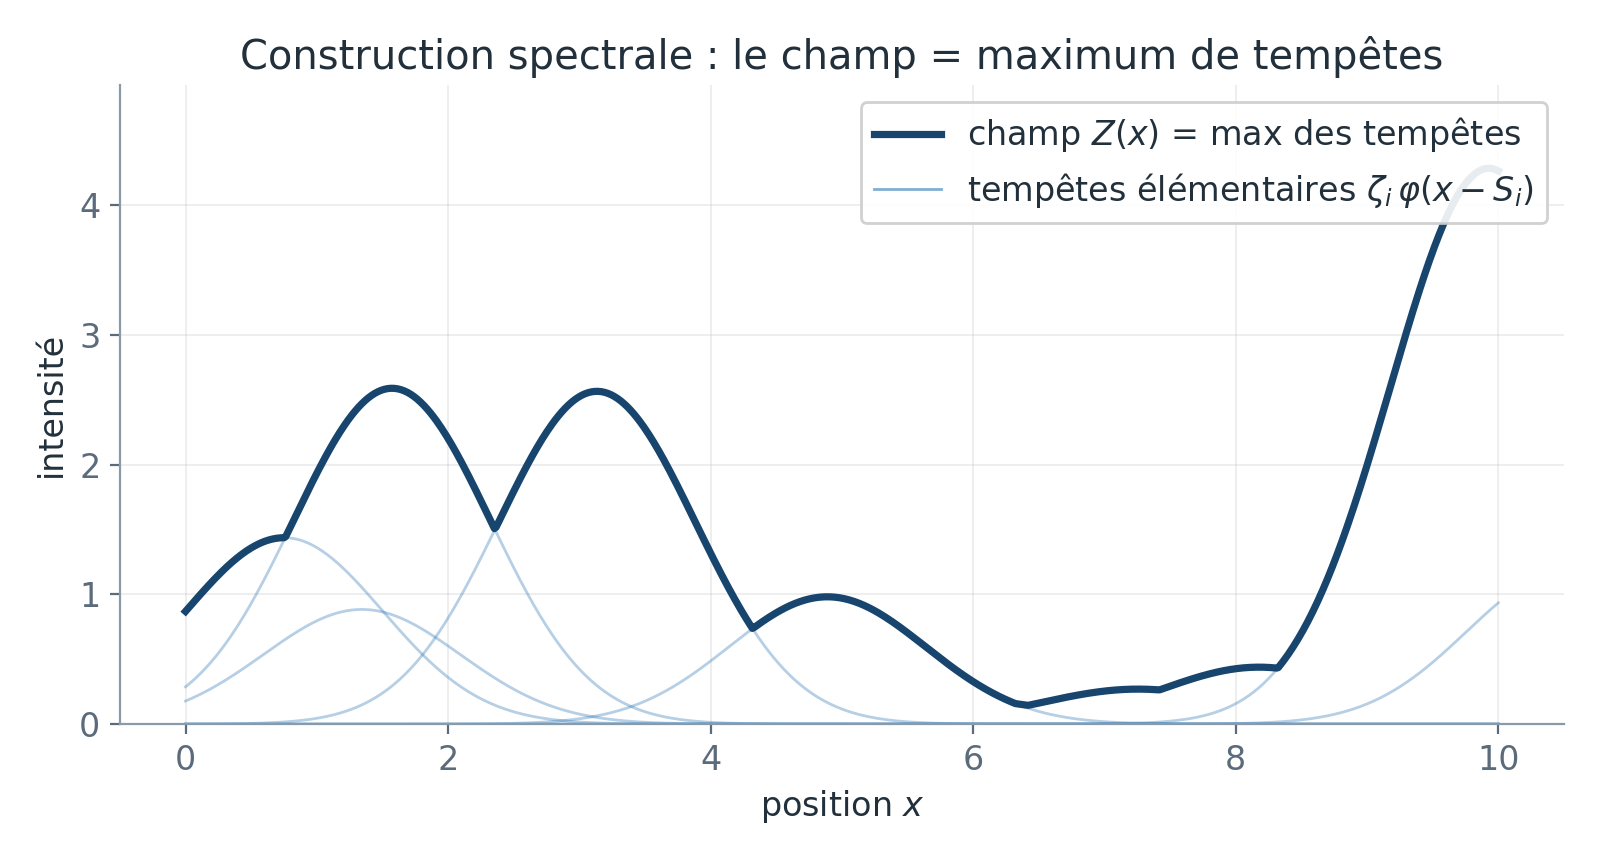
\includegraphics[width=0.82\linewidth]{figures/mamadou_figures/fig1_construction_spectrale_1d.png}
  \caption{Construction spectrale en dimension~1. Les courbes claires sont les
  tempêtes élémentaires $\zeta_i\,\varphi(x-S_i)$ ; la courbe foncée est le champ
  max-stable $Z(x)$, obtenu comme leur enveloppe supérieure (maximum point par
  point). En chaque position, le champ suit la tempête la plus haute.}
  \label{fig:spectral}
\end{figure}

La représentation~\eqref{eq:spectral} englobe deux classes classiques. Les
\emph{Mixed / Moving Maxima} (M3/M2) prennent une fonction de forme translatée
$V_{\mathbf x}(s)=f(\mathbf x-s)$ : chaque tempête est une même forme $f$ posée
en des points aléatoires. La \emph{représentation à base de processus
stochastiques} prend $V_{\mathbf x}=f(\mathbf x,\cdot)$, où la forme est
elle-même un processus aléatoire.

\subsection{Modèles paramétriques usuels}

Le choix de la fonction de forme définit le modèle. Le plus simple est le
\emph{modèle de Smith} : un processus M2 où la forme $f$ est la densité d'un
vecteur gaussien de covariance $\Sigma$. Chaque tempête est alors une
« cloche » gaussienne, et $\Sigma$ règle sa portée et son orientation. La
figure~\ref{fig:champ2d} en montre une réalisation en dimension~2 : les pics
lumineux sont les tempêtes dominantes.

\begin{figure}[htbp]
  \centering
  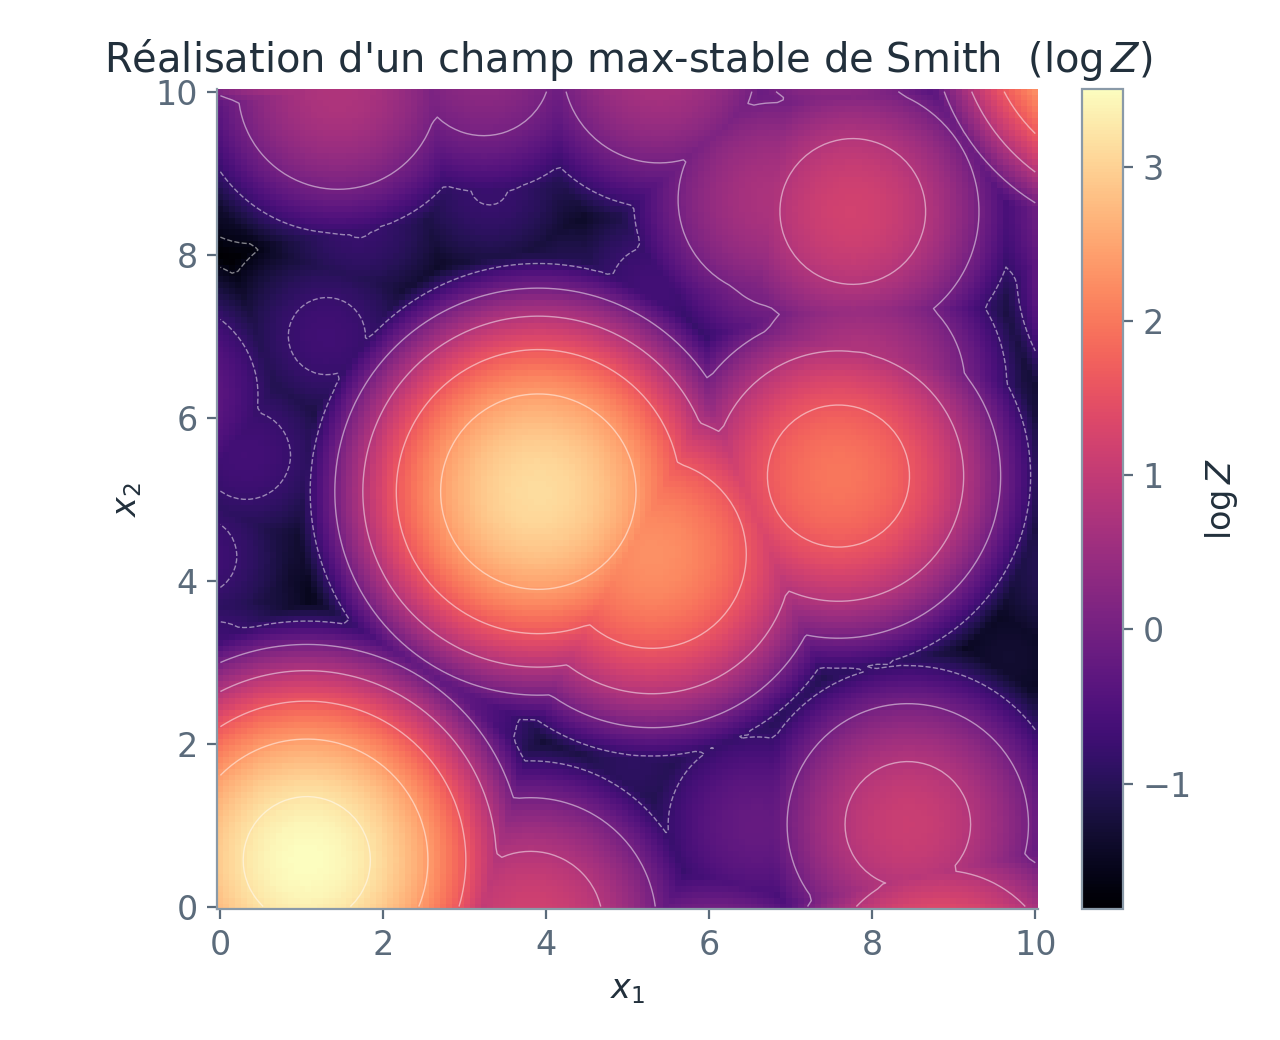
\includegraphics[width=0.62\linewidth]{figures/mamadou_figures/fig2_champ_smith_2d.png}
  \caption{Réalisation d'un champ max-stable de Smith en dimension~2
  ($\Sigma=I$), en échelle logarithmique. Chaque foyer clair correspond à une
  tempête gaussienne ; le champ est leur maximum ponctuel.}
  \label{fig:champ2d}
\end{figure}

D'autres modèles s'obtiennent par d'autres choix : le modèle de
\emph{Schlather} (forme à base d'un champ gaussien), le modèle de
\emph{Brown--Resnick} (fondé sur un variogramme) et le modèle \emph{tube}
(forme indicatrice sur un disque). Ces modèles reposent sur des fonctions de
corrélation isotropes $\rho$ dont la figure~\ref{fig:correl} présente trois
familles classiques ; les paramètres $c_1$ (portée) et $c_2$ (lissage)
contrôlent la vitesse et la régularité de la décroissance de la dépendance.

\begin{figure}[htbp]
  \centering
  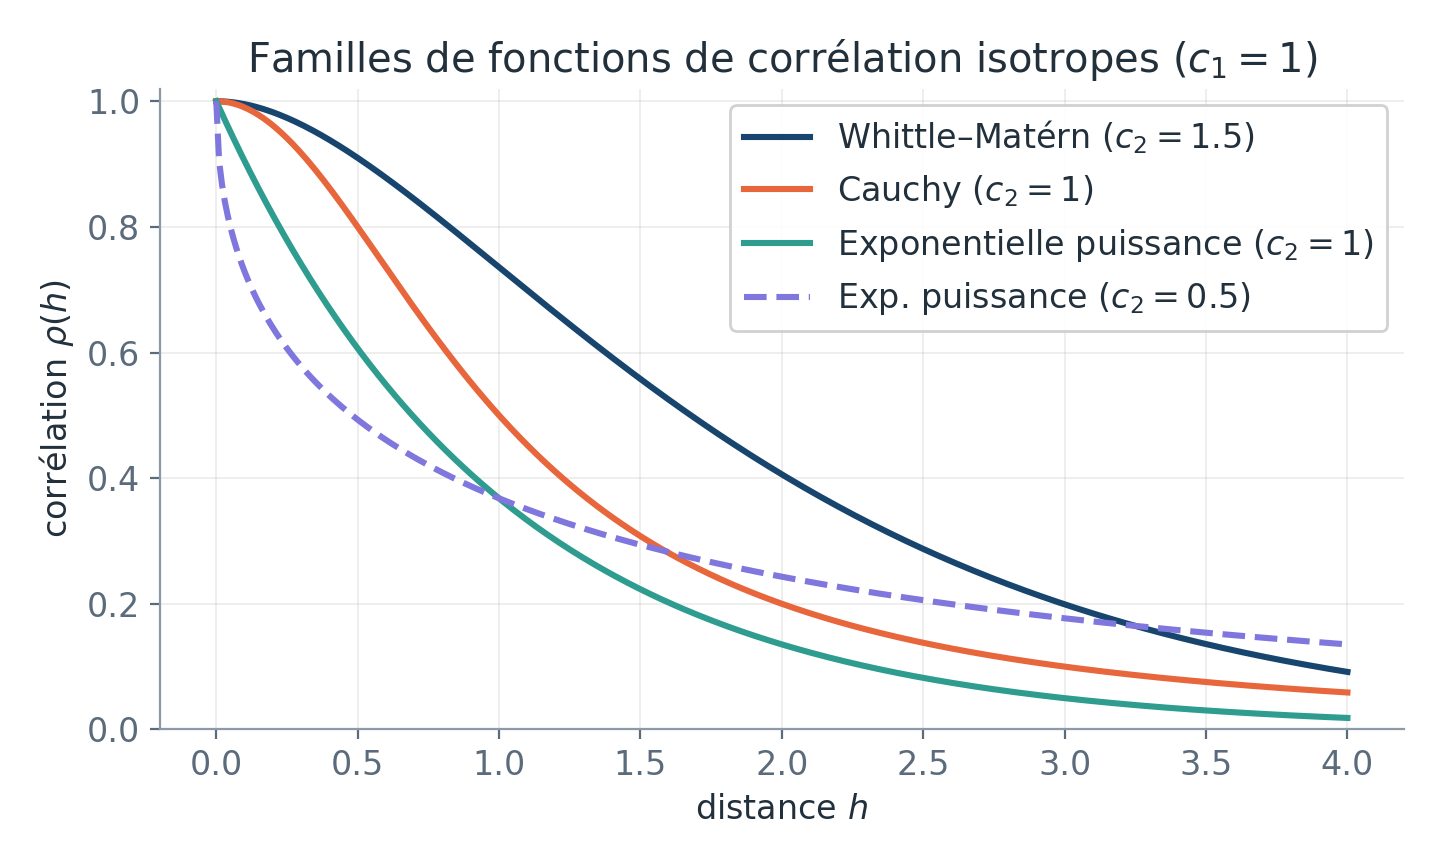
\includegraphics[width=0.78\linewidth]{figures/mamadou_figures/fig3_fonctions_correlation.png}
  \caption{Trois familles de fonctions de corrélation isotropes
  (Whittle--Matérn, Cauchy, exponentielle puissance), avec $c_1=1$. Elles
  gouvernent la structure de dépendance des modèles de Schlather,
  Brown--Resnick et gaussien géométrique.}
  \label{fig:correl}
\end{figure}

\subsection{Vers la dépendance spatiale}

La quantité qui résume la dépendance spatiale des extrêmes est le
\emph{coefficient extrémal} $\Theta$, défini par la loi bivariée
\begin{equation}\label{eq:theta-def}
\PP\bigl(Z(\mathbf x_1)\le u,\ Z(\mathbf x_2)\le u\bigr)
=\exp\!\left(-\frac{\Theta(\mathbf x_1,\mathbf x_2)}{u}\right),
\qquad \Theta\in[1,2].
\end{equation}
La valeur $\Theta=1$ correspond à la dépendance parfaite (les deux sites sont
extrêmes ensemble), $\Theta=2$ à l'indépendance. Pour un processus stationnaire
et isotrope, $\Theta$ ne dépend que de la distance
$h=\|\mathbf x_1-\mathbf x_2\|$, et croît de $1$ à $2$ à mesure que les points
s'éloignent (figure~\ref{fig:theta}). C'est cet objet, et son lien avec le
mélange (\emph{mixing}) du processus, qui gouverne la diversification spatiale
étudiée dans la partie suivante.

\begin{figure}[htbp]
  \centering
  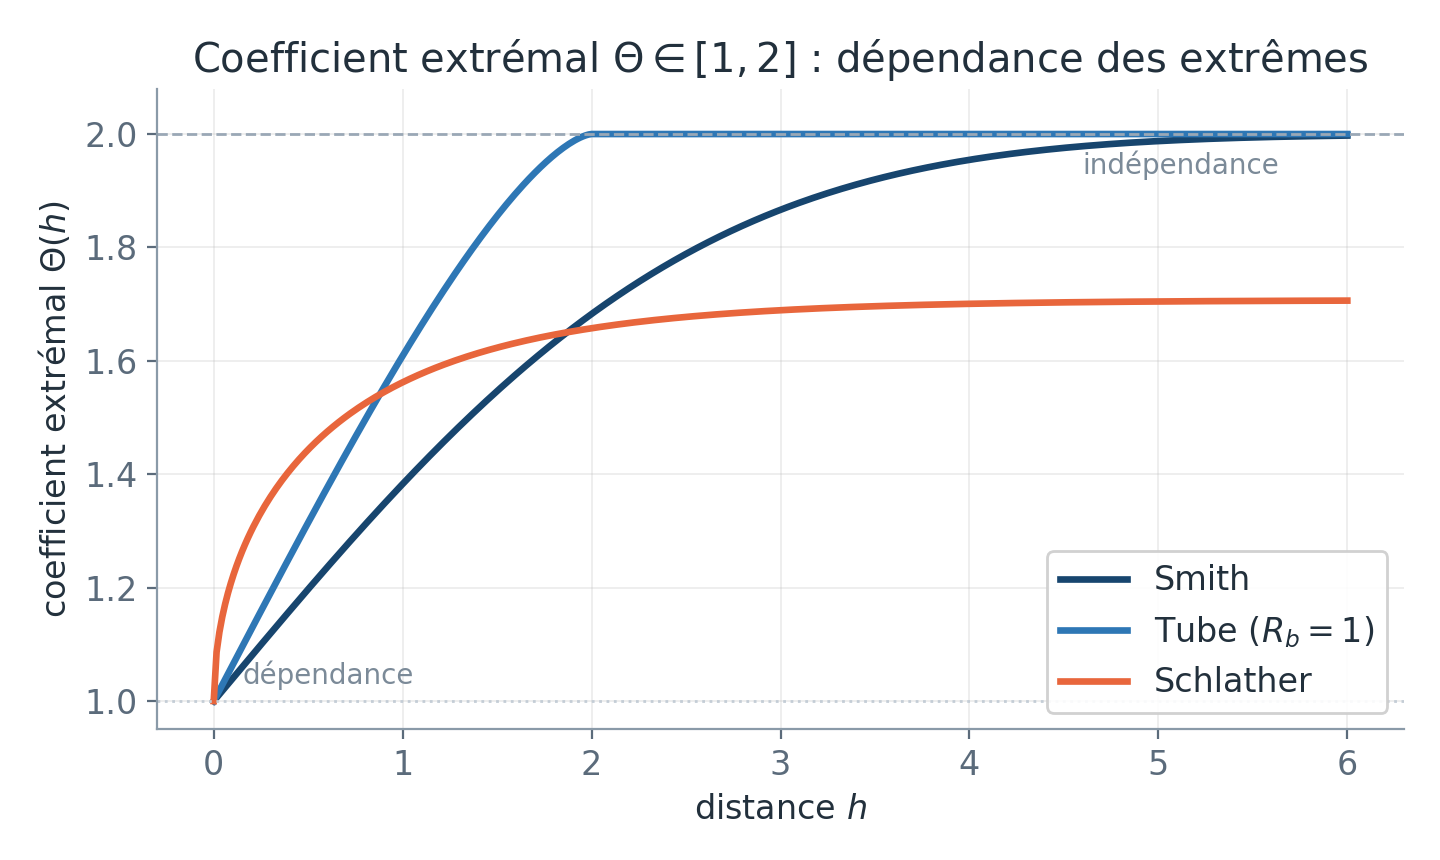
\includegraphics[width=0.78\linewidth]{figures/mamadou_figures/fig4_coefficient_extremal.png}
  \caption{Coefficient extrémal $\Theta(h)$ pour trois modèles. Il croît de la
  dépendance parfaite ($\Theta=1$) vers l'indépendance ($\Theta=2$) quand la
  distance augmente ; le modèle tube atteint l'indépendance à distance finie.}
  \label{fig:theta}
\end{figure}

